% Unofficial University of Cambridge Poster Template
% https://github.com/andiac/gemini-cam
% a fork of https://github.com/anishathalye/gemini
% also refer to https://github.com/k4rtik/uchicago-poster

\documentclass[final]{beamer}

% ====================
% Packages
% ====================

\usepackage[T1]{fontenc}
\usepackage{lmodern}
\usepackage[size=custom,width=120,height=72,scale=1.0]{beamerposter}
\usetheme{gemini}
\usecolortheme{cam}
\usepackage{graphicx}
\usepackage{booktabs}
%\usepackage[numbers]{natbib}
\usepackage{tikz}
\usepackage{pgfplots}
\pgfplotsset{compat=1.14}
\usepackage{anyfontsize}
\usepackage[style=numeric-comp,doi=false,url=false,isbn=false]{biblatex}
%\usepackage[doi=false,isbn=false,url=false]{biblatex}
\addbibresource{tom_biblatex.bib}
\renewcommand*{\bibfont}{\normalfont\small}

% ====================
% Lengths
% ====================

% If you have N columns, choose \sepwidth and \colwidth such that
% (N+1)*\sepwidth + N*\colwidth = \paperwidth
\newlength{\sepwidth}
\newlength{\colwidth}
\setlength{\sepwidth}{0.02\paperwidth}
\setlength{\colwidth}{0.176\paperwidth}

\newcommand{\separatorcolumn}{\begin{column}{\sepwidth}\end{column}}

% ====================
% Title
% ====================

\title{Einstein's Missing Energy}
\author{Thomas C. Andersen (nSCIr.ca Canada)}

% ====================
% Footer (optional)
% ====================

\footercontent{
  \href{https://nscir.ca}{https://nscir.ca} \hfill
  Quantum Gravity 2025 at Penn State July 21 - 25 \hfill ORCID: https://orcid.org/0000-0003-1614-4124 \hfill
  \href{mailto:tandersen@nscir.ca}{tandersen@nscir.ca}}
% (can be left out to remove footer)

% ====================
% Logo (optional)
% ====================

% use this to include logos on the left and/or right side of the header:
 \logoright{nscir.ca}
 \logoleft{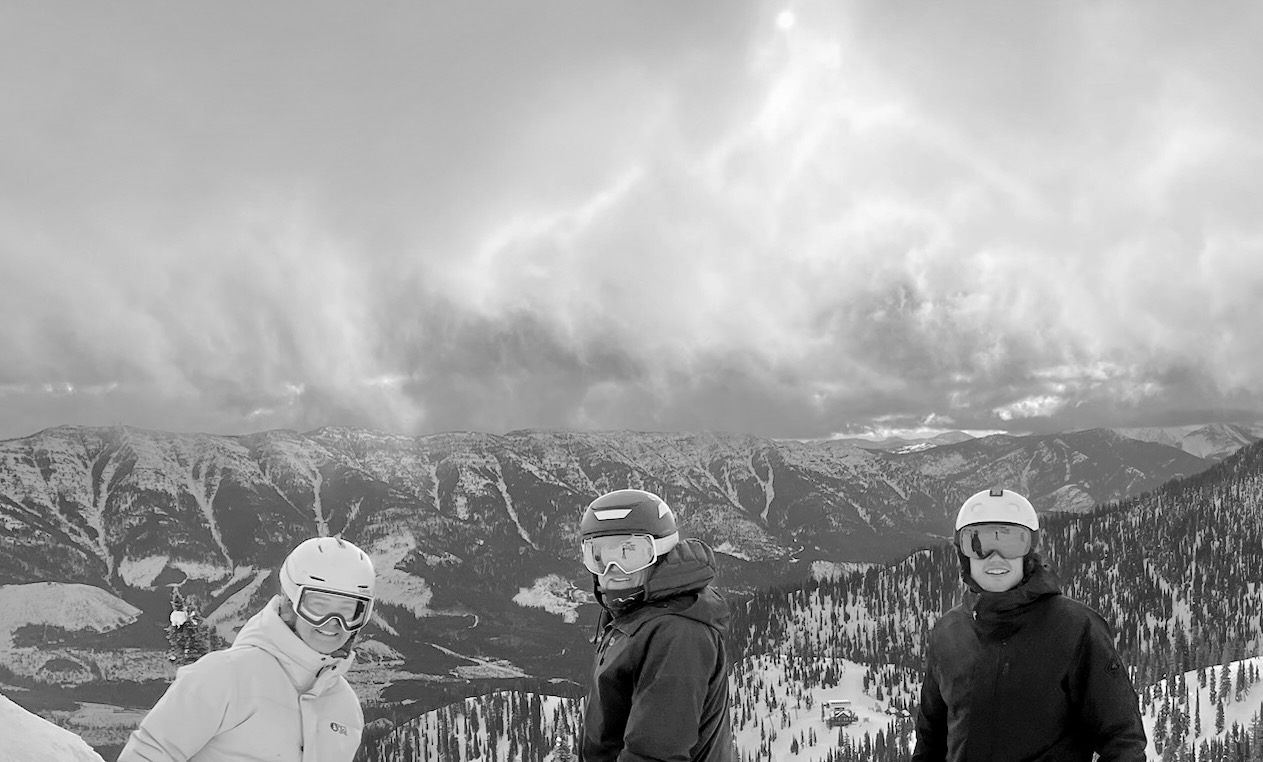
\includegraphics[height=5cm]{images/ski-fernie.jpeg}}

% ====================
% Body
% ====================

\begin{document}

% Refer to https://github.com/k4rtik/uchicago-poster
% logo: https://www.cam.ac.uk/brand-resources/about-the-logo/logo-downloads
%\addtobeamertemplate{headline}{}
%{
%    \begin{tikzpicture}[remember picture,overlay]
%      \node [anchor=north west, inner sep=3cm] at ([xshift=0.0cm,yshift=1.0cm]current page.north west)
%      {\includegraphics[height=4.5cm]{logos/cambridge-reversed-color-logo.eps}}; 
%    \end{tikzpicture}
%}

\begin{frame}[t]
\begin{columns}[t]
\separatorcolumn

% ============================================
% ============================================
%COLUMN 1
% ============================================
% ============================================

\begin{column}{\colwidth}
\begin{quotation}
Energy isn't conserved in General Relativity.
\end{quotation}
\rightline{\footnotesize --Will Kinney\cite{willkinney[@wkcosmo]EnergyIsntConserved2021}}

\begin{quotation}
actual physics is non-local.
\end{quotation}
\rightline{\footnotesize --Tim Maudlin\cite{Maudlind}} 



  \begin{block}{Abstract}
In this poster we restore energy conservation in General Relativity, which for our theory, implies a universal rest frame. The solution presented here thus drops covariance, but regular (think Standard Model) matter and energy still behave covariantly. As an example, a Schwarzschild like solution is developed within our framework, using Birkhoff's theorem. Unlike a black hole, this solution shows no horizons and no massive singularity. We also find a new polarization mode of gravitational radiation, namely (superluminal!) monopolar radiation.

The new theory has some parallels with Quantum mechanics, which is known to prefer an absolute time (via the Schrödinger equation) and non - local physics (through Bell violations).

Thus, we begin a journey to emerge quantum mechanics from a new extension of Einstein's General Relativity that obeys Emily Noether's energy conservation. 

  \end{block}

  \begin{block}{Ad Hoc energy conservation}
  	We know gravitational energy certainly exists, and does impact the total energy of a space time. For example, with gravitational waves (imagine near a coalescing binary black hole), researchers simply plop the wave energy into the right side stress energy tensor. But you can't always do it - there is no reliable, 'energy is built in' theory. That's the point. Einstein (and everyone else) couldn't get that to work. Indeed, it probably can't work, although lots of people have tried.

  \end{block}

  \begin{block}{Pseudo Tensors}


Einstein and others hope to fix this lack of energy conservation lay in `pseudo tensors', which are discussed and evaluated for example by Virbhadra\cite{virbhadraEnergyDistributionKerrNewman1990}\cite{virbhadraEnergyMomentumVaidya1992}. It's fairly straight forward using Mathematica to see how unreliable these pseudo tensors are - the same physical Schwarzschild solution in isotropic $x,y,z,t$ vs `Kerr-Schild' in $x,y,z,t$ give conflicting results\cite{RzeroMathematicaSchwarschildpseudoChecknb}. Pseudo tensors don't work.
  \end{block}

  \begin{block}{Quasi Local Energy}
There are improvements to be had over the pseudo tensor approach. The quasilocal energy of Brown and York\cite{Brown1993} and Katz\cite{Katz2005} and others \cite{haroNoethersTheoremsEnergy2021}\cite{lyndenbell1985}\cite{changPseudotensorsQuasilocalEnergymomentum1999} detail how to assign energy to the gravitational field. 

These treatments crucially don't take the step of letting the gravitational field know about this energy. It's viewed as a curiosity of an existing (say vacuum) solution. 
  \end{block}


\end{column}

\separatorcolumn

% ============================================
% ============================================
%COLUMN 2
% ============================================
% ============================================

\begin{column}{\colwidth}
  \begin{block}{The Theory: Energy Conservation}
We put the energy of the gravitational $Q(F)$ , where $F$ represents the gravitational field, into the Einstein equations as a new separate term: 
  \begin{equation}
R_{\mu\nu}-\dfrac{1}{2}g_{\mu\nu}R - Q(F) = 8\pi G T_{\mu \nu}.
\label{newEquation}
\end{equation}
	$Q(F) \approx 0$ if the gravitational field is in the linear regime. So for regular matter (say solar system and earth lab dynamics), it's ignorable. 
	
	However, in a strong gravity situation we would have to \textit{account for the mass generated by the energy content of that space time}.
\end{block}
  
  \begin{block}{Example: Spherical Symmetry }
 We now build a Schwarzschild like solution that includes gravitational energy, using quasilocal energy, which in the Schwarzschild solution is (far field, with isotropic r)\cite{lyndenbell1985}: 

\begin{equation} \label{energyDensityEqn}
	E_{density} = \frac{Gm(r)^2}{8 \pi r^4}.
\end{equation}
To obtain the mass function $m(r)$: we start at a distant point out where $m(r) = M$, then walk in, dropping some energy from the Birkhoff mass at r into the gravitational field at every step, thus allowing this energy to build the gravitational field.
	
A python script\cite{RzeroJupyterGravitationalEnergyipynb} easily numerically calculates the mass function, which turns out to be (in isotropic coords)

\begin{equation}
	m(r) = M - M/(1 + 2r/M).
\end{equation}

The resulting metric is then:
		\begin{equation} \label{lineElement}
			ds^2 = \frac{-r^2}{(M+r)^2}dt^2 + \frac{16(M+r)^4}{(M+2r)^4}(dr^2 + r^2d\theta^2 + r^2 sin^2(\theta)d\phi^2),
		\end{equation}

which shows no singularity. The energy required to build the gravitational field is exactly equal to the distant mass M of the object. Simple.
\end{block}

\begin{alertblock}{Confusion on Gravitational Energy}

The literature on the subject of `where the energy is' - even for the Schwarzschild solution - full of contradictions. The energy is outside or inside the horizon, positive or negative, 2M, or M, or zero, etc.  For example, D. Lynden-Bell and Katz on the localization of mass:\cite{lyndenbell1985}

\begin{quotation}
	The Penrose mass of a Schwarzschild hole is all within the hole, whereas ours is all outside it.
\end{quotation}

We believe that much of the confusion arises from double counting the mass/energy in the Schwarzschild solution, both the field and the point mass contribute, leading authors to awkward choices. 

\end{alertblock}


\end{column}

\separatorcolumn

% ============================================
% ============================================
%COLUMN 3
% ============================================
% ============================================

\begin{column}{\colwidth}

  \begin{exampleblock}{No Singularity}

    \begin{figure}
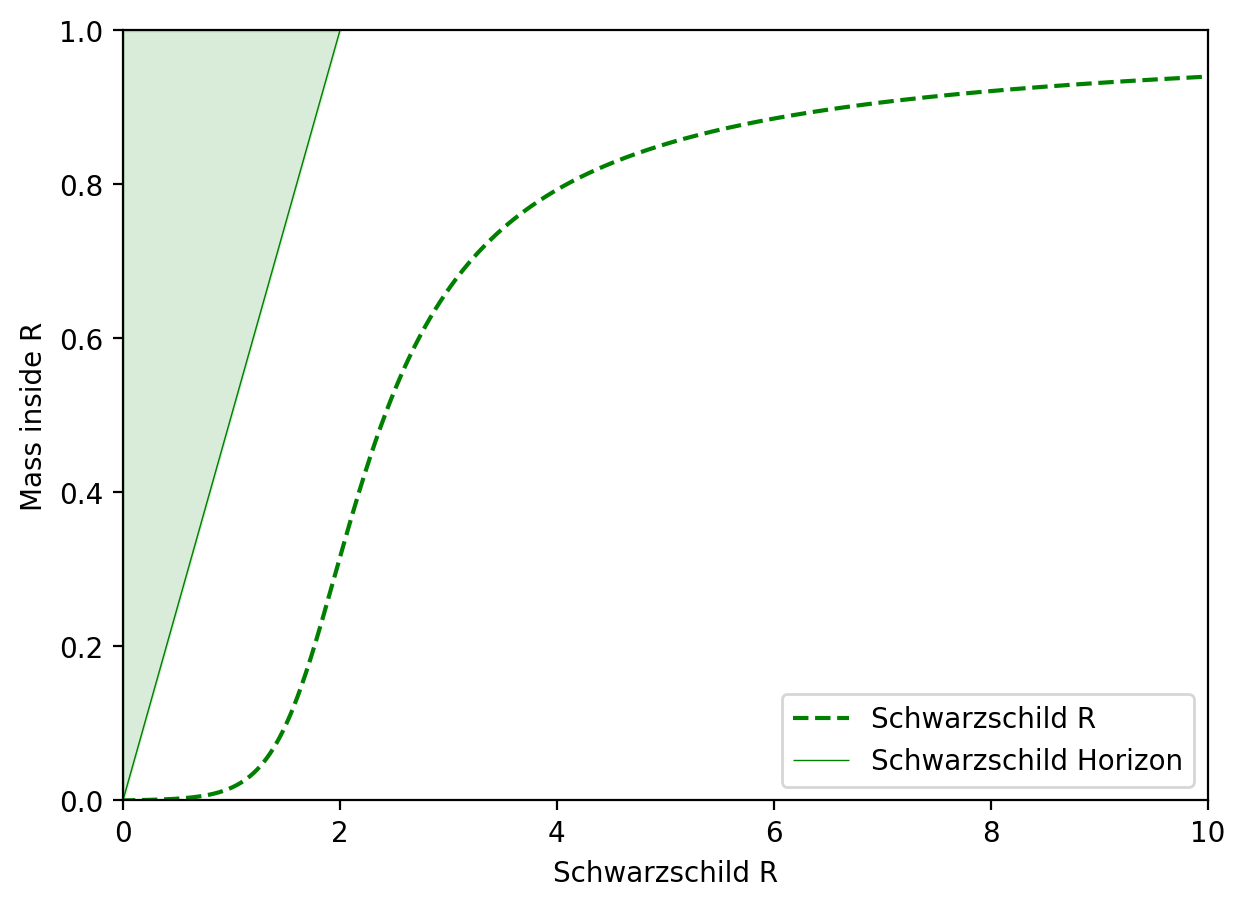
\includegraphics[width=0.9\columnwidth]{no-horizons-s.png}
\caption{The mass function as found here, in Schwarzschild coordinates. The mass at every radius is below the horizon radius for that mass, so there is no event horizon. Also one can see that the behaviour as $r \rightarrow 0$ is not a problem. For a normal black hole, the mass function is a horizontal line at the top of the graph, at M = 1. A neutron star has a radius of $\approx 5$ on this graph.}
\label{isotropic-energy-hole-s}
\end{figure} 

\end{exampleblock}

\begin{block}{Monopole Superluminal Waves}
	We will look at what happens in our solution in the case of a small perturbation in the mass at r. 
\begin{figure}
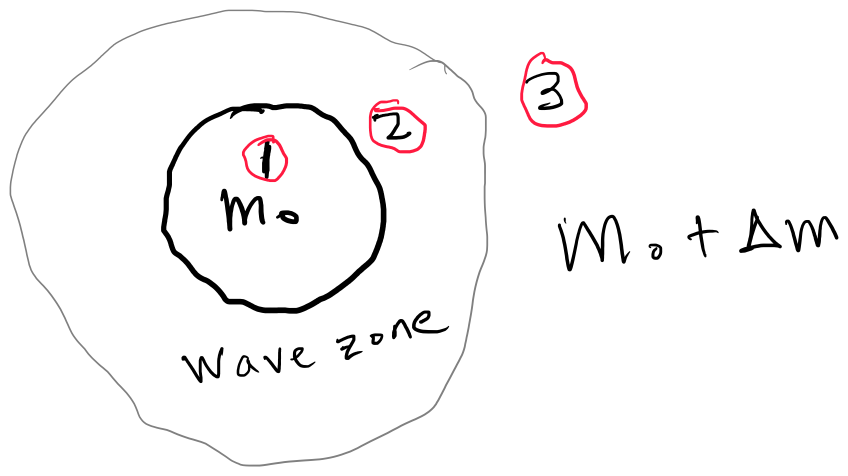
\includegraphics[width=0.45\columnwidth]{monopole.png}
\caption{Monopole Wave: There are three zones. Inner zone: a Schwarzschild region with mass $M_0$. Outer zone an implied mass of $M_o + \Delta M$. In between is the 'wave zone' where the perceived mass drops. Almost all the drop is near the boundary wall at $r$ between \textbf{1} and \textbf{2}. We will find that this boundary must be rapidly moving to satisfy global energy conservation.}
\label{monopoleEnergy} 
\end{figure}

The problem with energy conservation here is immediately apparent. An observer in the outer zone will, by Birkhoff's theorem, see a total mass of $M_o + \Delta M$ - but this extra mass $\Delta M$ is not actually there. We fix it by giving the wave zone a velocity, and using its kinetic energy to balance the books. See\cite{andersenEinsteinsMissingEnergy2025}.

\begin{equation} \label{finalSpeedEqn}
 v = \sqrt{\frac{2 r}{GM} - 2}.
\end{equation}

Equation (\ref{finalSpeedEqn}) is the speed at which a monopolar wave would need to travel. It usually works out to a value of tens of thousands of times the speed of light. The wave slows as the gravitational well increases in depth. It has the exact same form as the formula for the speed of a tsunami: $\sqrt depth$. These monopole waves feel the global structure.
\end{block}


\end{column}
\separatorcolumn

% ============================================
% ============================================
%COLUMN 4
% ============================================
% ============================================

\begin{column}{\colwidth}
  \begin{block}{Quantum Mechanics}
  
  Emergent Quantum Mechanics postulates that quantum mechanics arises from de Broglie - Bohm like mechanics based on a real (often scalar) field\cite{Bush2015a}. We speculate that the Faraday waves of Emergent Quantum Mechanics may be the monopole waves postulated here. 
  
  Quantum mechanics has problems with relativity and also has non local effects. We are investigating if the superluminal aspect of the monopole waves discussed here can be a mechanism for quantum non locality. Experiments to determine the 'speed of spooky quantum action at a distance'\cite{salartTestingSpeedSpooky2008a} have determined minimum speeds of the same order of magnitude as equation (\ref{finalSpeedEqn}).
   
From the earth and sun on earth's surface:
  \begin{equation}
 v_{earth} = \sqrt{\frac{2*6000km}{1 cm} - 2} \ \approx 35000c ,
\end{equation}
\begin{equation}
 v_{sun} = \sqrt{\frac{2*150e6km}{3 km} - 2} \ \approx 10000c . 
\end{equation}

      \begin{figure}
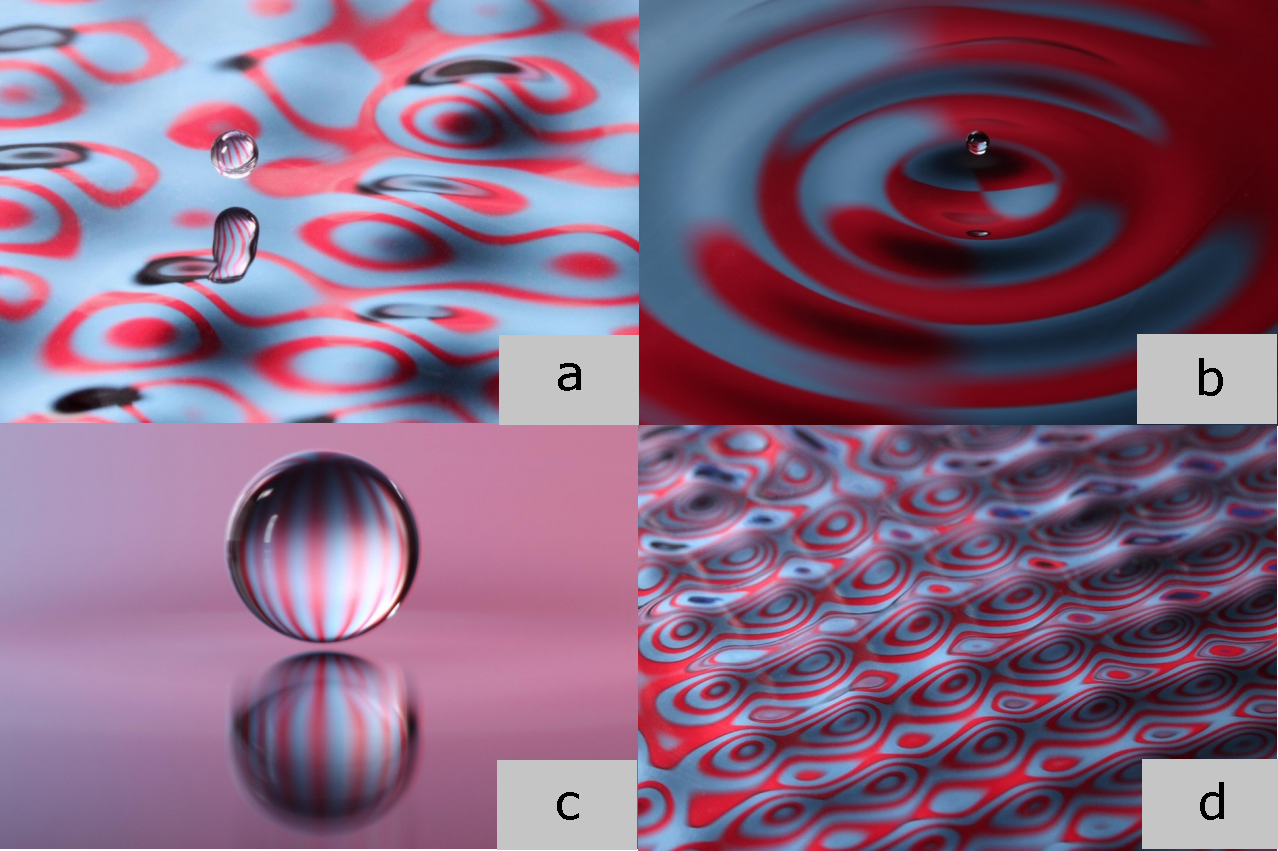
\includegraphics[width=0.9\columnwidth]{bush-waves.png}
\caption{Some visualizations of Pilot wave - Faraday waves. (Creative commons). \cite{Bush2015a}}
\label{bush-faraday}
\end{figure} 

  
\begin{exampleblock}{Experimental tests}

Explain it.
\end{exampleblock} 
   
\end{block}



\end{column}
\separatorcolumn
% ============================================
% ============================================
%COLUMN 5
% ============================================
% ============================================

\begin{column}{\colwidth}

  \begin{alertblock}{Summary}
    \begin{itemize}
      \item \textbf{Normal Physics:} light and matter use the exact same normal Einstein Equations of GR.
      \item \textbf{Adding Energy Conservation} requires breaking covariance, which we do by picking a frame.
      \item \textbf{Schwarzschild} like solutions have no singularities.
       \item \textbf{Quasi-local energy} is unambiguous and adds to M.
       \item \textbf{Monopolar waves} can exist and travel at ~10,000c.
       \item \textbf{Special Relativity} is assumed to be in the Lorentz/Poincarie method, where a single stationary frame is postulated.
       
    \end{itemize}
  \end{alertblock}

\begin{block}{References}
\printbibliography
\end{block}

\end{column}


\separatorcolumn
\end{columns}
\end{frame}

\end{document}
